\documentclass[15pt,a5paper,reqno]{article}
\usepackage{hyperref}
\usepackage[warn]{mathtext}
\usepackage[utf8x]{inputenc}
\usepackage{amssymb, amsmath, multicol}
\usepackage[russian]{babel}
\usepackage{graphicx}
\usepackage[shortcuts,cyremdash]{extdash}
\usepackage{wrapfig}
\usepackage{floatflt}
\usepackage{lipsum}
\usepackage{verbatim}
\usepackage{concmath}
\usepackage{euler}
\usepackage{xcolor}
\usepackage{etoolbox}
\usepackage{fancyhdr}
\usepackage{subfiles}
\usepackage{enumitem}
\usepackage{amsthm}
\usepackage{indentfirst}
\usepackage{import}

\DeclareMathOperator{\sign}{sign}

\RequirePackage[ left     = 1.5cm,
  right    = 1.5cm,
  top      = 2.0cm,
  bottom   = 1.25cm,
  includefoot,
  footskip = 1.25cm ]{geometry}
\setlength    {\parskip}        { .5em plus .15em minus .08em }
%\setlength    {\parindent}      { .0em }
\renewcommand {\baselinestretch}{ 1.07 }

\fancyhf{}

\renewcommand{\footrulewidth}{ .0em }
\fancyfoot[C]{\texttt{\textemdash~\thepage~\textemdash}}
\fancyhead[R]{\hfilШурыгин}

\makeatletter
\patchcmd\l@section{%
  \nobreak\hfil\nobreak
}{%
  \nobreak
  \leaders\hbox{%
    $\m@th \mkern \@dotsep mu\hbox{.}\mkern \@dotsep mu$%
  }%
  \hfill
  \nobreak
}{}{\errmessage{\noexpand\l@section could not be patched}}
\makeatother
\parindent = 1cm % отступ при красной строке⏎
\pagestyle{fancy}    
\renewcommand\qedsymbol{$\blacksquare$}

\newcommand{\when}[2]{
  \left. #1 \right|_{#2} \hspace
}
\renewcommand{\kappa}{\varkappa}
\RequirePackage{caption2}
\renewcommand\captionlabeldelim{}
\newcommand*{\hm}[1]{#1\nobreak\discretionary{}

\DeclareSymbolFont{T2Aletters}{T2A}{cmr}{m}{it}
{\hbox{$\mathsurround=0pt #1$}}{}}
% Цвета для гиперссылок
\definecolor{linkcolor}{HTML}{000000} % цвет ссылок
\definecolor{urlcolor}{HTML}{799B03} % цвет гиперссылок
 
\hypersetup{pdfstartview=FitH,  linkcolor=linkcolor,urlcolor=urlcolor, colorlinks=true}


%\setcounter{secnum[utf8x]depth}{0}

\begin{document}

% НАЧАЛО ТИТУЛЬНОГО ЛИСТА
\begin{center}
  {\small ФЕДЕРАЛЬНОЕ ГОСУДАРСТВЕННОЕ АВТОНОМНОЕ ОБРАЗОВАТЕЛЬНОЕ\\ УЧРЕЖДЕНИЕ ВЫСШЕГО ОБРАЗОВАНИЯ\\ МОСКОВСКИЙ ФИЗИКО-ТЕХНИЧЕСКИЙ ИНСТИТУТ\\ (НАЦИОНАЛЬНЫЙ ИССЛЕДОВАТЕЛЬСКИЙ УНИВЕРСИТЕТ)\\ ФИЗТЕХ-ШКОЛА РАДИОТЕХНИКИ И КИБЕРНЕТИКИ}\\
  \hfill \break
  \hfill \break
  \hfill \break
  \Huge{Интерферометр Майкельсона}\\
\end{center}

\hfill \break
\hfill \break
\hfill \break
\hfill \break
\hfill \break
\hfill \break

\begin{flushright}
  \normalsize{Работу выполнил:}\\
  \normalsize{\textbf{Шурыгин Антон Алексеевич, группа Б01-909}}\\
\end{flushright}

\begin{center}
  \normalsize{\textbf{Долгопрудный, 2021}}
\end{center}


\thispagestyle{empty} % выключаем отображение номера для этой страницы

% КОНЕЦ ТИТУЛЬНОГО ЛИСТА

\newpage
\thispagestyle{plain}
\tableofcontents
\thispagestyle{plain}
\newpage


\textbf{Цель работы:} Изучение двухлучевой интерференции, определение длины волны, проверка эффекта Доплера.

\textbf{Оборудование:} интерферометр Майкельсона с подвижным зеркалом, лазер, фотоумножитель, частотомер, линзы.

\section{Введение и краткая теория}

Интерферометр Майкельсона находит применение в спектрометрах с высоким разрешением, для абсолютных и относительных измерений длин с точностью 0,005 мкм. 

Оптическая схема интерферометра приведена на рис. 1. Источником света служит лазер $ЛГ$. Лазер излучает узкий пучок света, который фокусируется линзой Л1. В фокусе этой линзы возникает точечный
источник света S. Сферическая световая волна от источника S падает на делительный кубик ДК и делится его диагональной гранью на 
две волны — отражённую $1$ и проходящую $2$. Волна 1 отражается от
зеркала $З_1$, возвращается к кубику, частично проходит сквозь него и
попадает на экран $Э$. Волна $2$ отражается от зеркала $З_2$, частично отражается от кубика и также попадает на экран. Световые волны $1$ и $2$
испускаются одним источником S, и они когерентны между собой. Эти
волны создают на экране $Э$ интерференционную картину. Для увеличения масштаба интерференционной картины может быть использована
линза $Л_2$.

Зеркало З1 установлено перпендикулярно падающему лучу. Оно может перемещаться вдоль луча. Это зеркало в дальнейшем будет называться подвижным. Зеркало З2 вдоль направления падающего луча не
перемещается. Его, однако, можно наклонять по отношению к лучу.

\begin{figure}[h!]
    \centering
    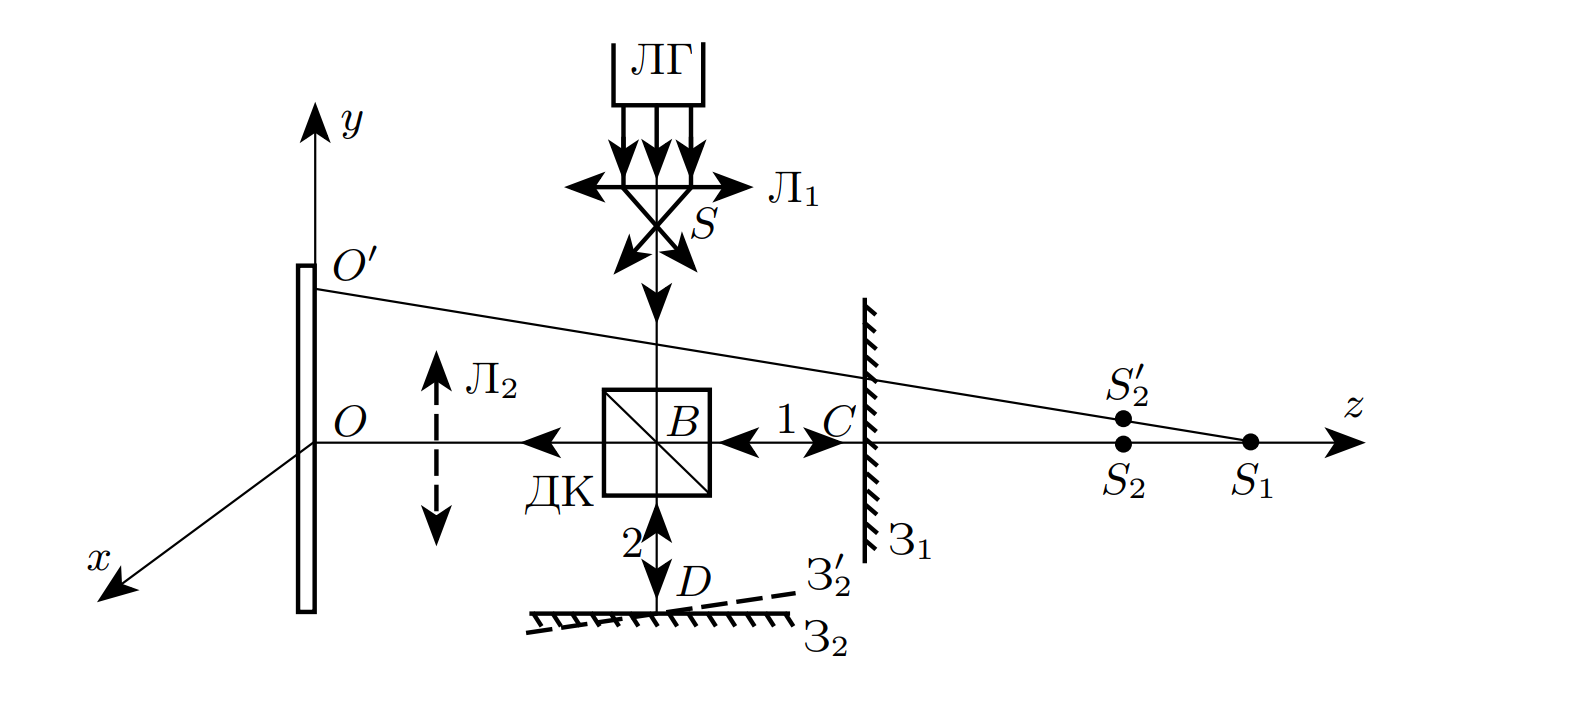
\includegraphics[width=1.2\linewidth]{pics/scheme.png}
    \caption{Схема интерферометра}
    \label{}
\end{figure}


\section{Схема установки}


Схема экспериментальной установки приведена на рис. 2. Источником света служит гелий-неоновый лазер
ЛГН-203. Его излучение обладает большой длиной когерентности, что
позволяет получать хорошо различимую глазом интерференционную
картину при разности хода в десятки сантиметров. Неподвижное зеркало З2, поворачивается микрометрическими винтами Мг (относительно горизонтальной) и Мв (относительно вертикальной оси). Зеркало З1
установлено перпендикулярно падающему лучу. Оно может передвигаться вдоль луча с помощью микрометрического винта, соединённого
с двигателем Дв через муфту и редуктор РД, позволяющий менять
скорость движения зеркала. Двигатель питается от сети через блок питания пульта управления. Концевые контакты К1 и К2 меняют направление движения зеркала на обратное. Включение лазера и двигателя
производится с пульта управления. Сигнальные лампочки указывают,
в какую сторону движется зеркало.

Интерференционная картина наблюдается на экране Э. Она может
быть увеличена с помощью линзы Л2. В этом случае на экране в увеличенном масштабе воспроизводится интерференционная картина, которая создаётся перед линзой в плоскости, сопряжённой экрану. Линза
закреплена на съёмном столике, её фокусное расстояние 4,3 см.


Для регистрации изменения интенсивности света используется фотоэлектронный умножитель ФЭУ-68, установленный непосредственно
за экраном. Свет на окно ФЭУ попадает через небольшое отверстие в
центре экрана. Для питания ФЭУ используется высоковольтный выпрямитель. Выпрямитель включается тумблером «Сеть» на пульте управления.
Периодическое изменение интенсивности света, возникающее при
движении зеркала З1, приводит к такому же изменению сигнала ФЭУ.

Число периодов изменения интенсивности света пересчитывается частотомером Ч3-54. Частотомер может работать в одном из трёх режимов.

\begin{enumerate}
    \item Он может измерять число импульсов, поступающих на его входы
    (А или Б) за некоторый промежуток времени (его продолжительность
    определяется поступлением сигналов на управляющие входы В и Г).

    \item С помощью частотомера можно измерять промежутки времени.
    Для таких измерений в прибор встроен кварцевый генератор. Частотомер измеряет время, прошедшее между поступлением сигналов на его
    управляющие входы, подсчитывая соответствующее число импульсов кварцевого генератора
    
    \item Наконец, частотомер может измерять частоту сигнала, поступающего на его вход, сравнивая число периодов исследуемого сигнала с
    числом импульсов кварцевого генератора.
\end{enumerate}


Для получения управляющих сигналов используется геркон $Г$ (герметичный магнитоуправляемый контакт). Схема работает следующим
образом. На отсчётной головке микрометрического винта зеркала $З_1$
закреплён небольшой магнит. Головка вращается вместе с винтом. После срабатывания концевого контакта $К_1$ зеркало начинает двигаться
к экрану. При приближении магнита к геркону вырабатывается управляющий сигнал, который подаётся через схему пульта управления на
вход В частотомера. Частотомер начинает счёт импульсов. Сигнал на
окончание счёта подаётся на вход $Г$ после того, как с помощью геркона зарегистрировано $3_2$ оборота ходового винта. После срабатывания
концевого контакта $K_2$ зеркало начинает движение от экрана. На этом
участке движения счёт импульсов не производится. Один оборот микрометрического винта приводит к перемещению зеркала на $1$ мм. Таким
образом, полное перемещение зеркала $З_1$ составляет $L = 32 \text{  мм}$.

\begin{figure}[h!]
    \centering
    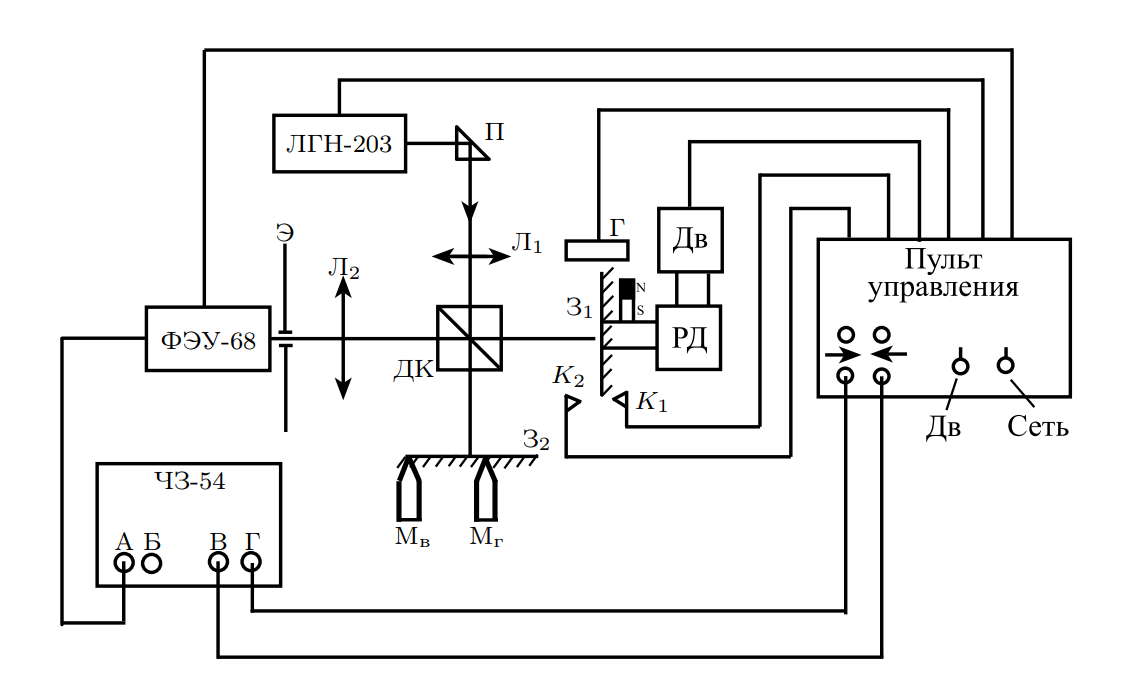
\includegraphics[width=1.1\linewidth]{pics/lab_scheme.png}
    \caption{Схема интерферометра}
    \label{}
\end{figure}


\section{Ход работы}


\subsection{Исследование интерференционной картины}


Совместим центр креста с центром колец, наметим положение 5–6-ти
первых тёмных колец и измерьте их диаметры.

Убедимся в справедливости формулы:

\[ r_n \approx \sqrt{\frac{2nL(L-a)}{m_0}}  \]


Для этого построим график зависимости квадрата радиуса кольца от его номера. По наклону полученной прямой найдём величину $\frac{L(L − a)}{m_0}$. Сравним найденное число с результатом теоретического расчёта. 

Таким образом, получаем, что величина $\frac{2L(L − a)}{m_0} \approx 0.2$.

Согласно рис. 1,
\[ L = OS_1 = BS_1 + OB , \:\:\:\:\: L − a = OS_2 = BS_2 + OB \]
\[ BS_1 = 2\cdot BC + SB, \:\:\:\:\: BS_2 = 2\cdot BD + SB \]
 
 Проведите расчёт, принимая $SB$ = 5 см, $BC$ = 26 см
(для среднего положения зеркала), $BD$ = 22 см, расстояние от делительного кубика до линзы $Л_2$ — 16,5 см, расстояние от линзы до экрана — 15 см, фокусное расстояние линзы $Л_2$ — 4,3 см.

Кроме того, порядок интерференции равен: 

\[    m_0 = \frac{a}{\lambda}           \]

Причем $a$ - это расстояние между изображениями источника $S$ на экране, она же разность хода между лучами 1 и 2.

Разность хода в интерферометре Майкельсона определяем как удвоенная разность плеч:

\[    a = 2 \cdot (BC - BD)  = 8 \text{  cm}  \]

%%Тогда $ m_0 = \frac{a}{\lambda} = \frac{4}{6328 \cdot 10^{-8} \approx 63211 $  

Тогда $m_0  \approx $ 125000. 

$ L =  2\cdot BC + SB + OB = 2 \cdot 26 + 5 + 16.5 + 15 = 88.5$ cm.

$ L - a = 2\cdot BD + SB + OB = 2 \cdot 22 + 5 + 16.5 + 15 = 80.5 $ cm.

Таким образом, получаем что: 

\[    \frac{2\cdot 88.5 \cdot 80.5}{125000} \approx  0.13   \]

Получим на экране картину вертикальных полос. Для этого уведите
центр пятна в сторону по горизонтали ($O \rightarrow O′$ на рис. 1), сместив микрометр $М_в$ на $0,08–0,09$ мм от исходного положения. Измерим ширину
полосы в центре экрана (в т. O) и расстояние O′O на экране. Зная $OS_1$,
оцените угол поворота зеркала и смещение изображения источника света ($S_2S_2′$).
Угол поворота зеркала вдвое меньше угла $\frac{OO′}{OS_1}$.



\begin{figure}[h!]
  \centering
  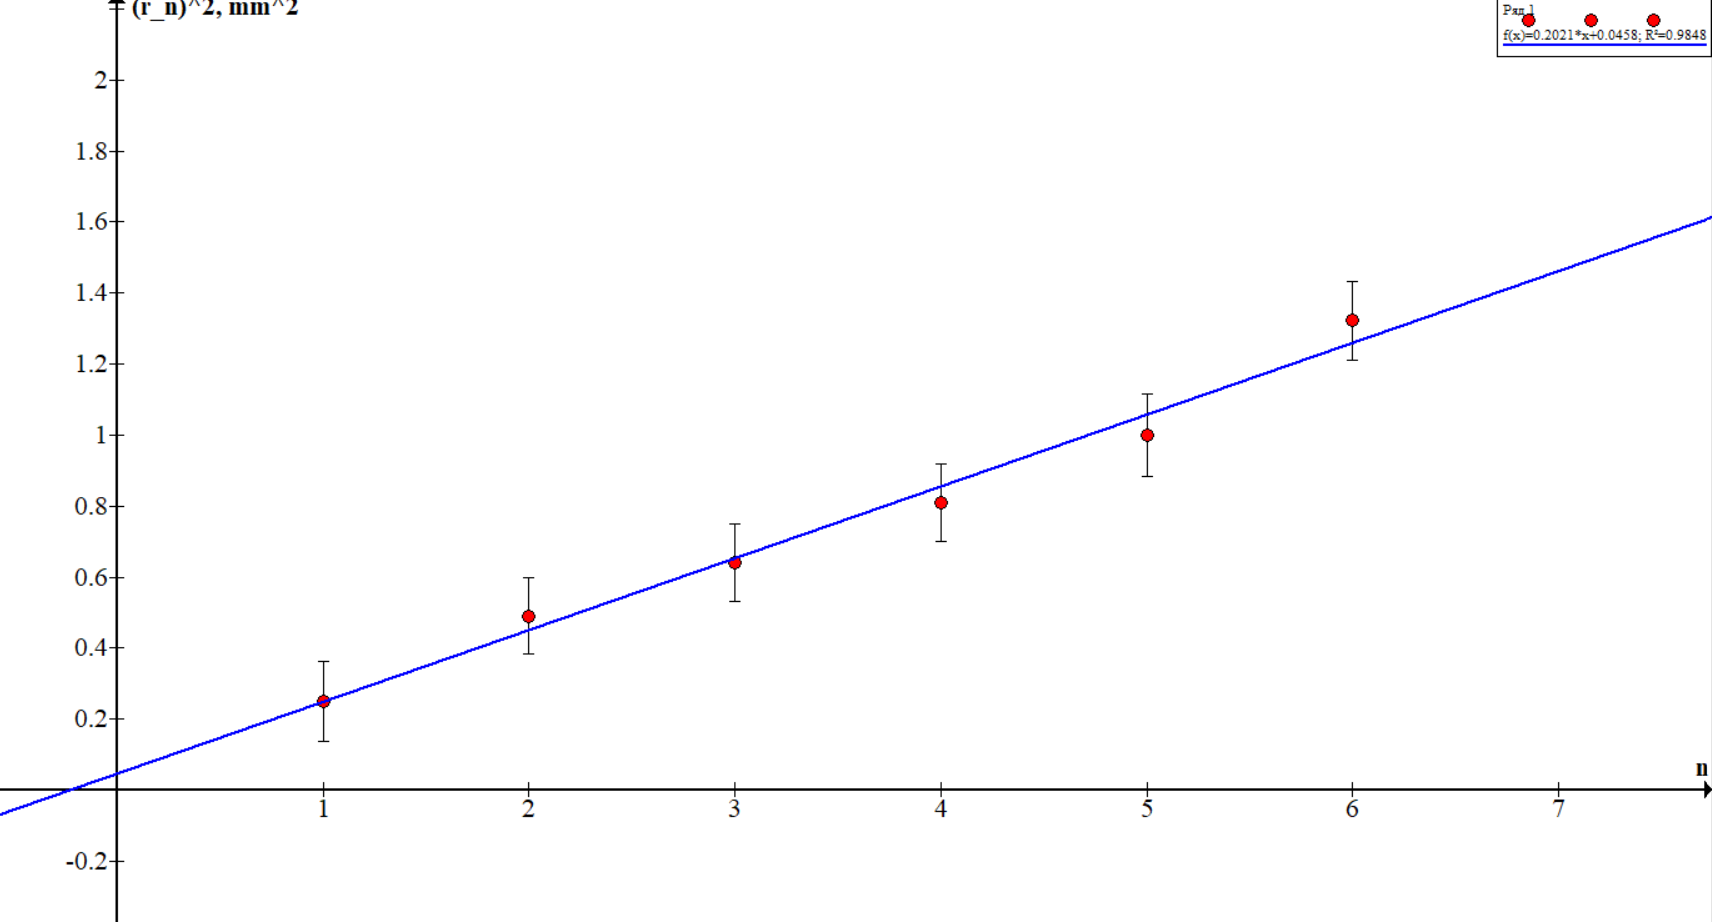
\includegraphics[width=1\linewidth]{pics/lab_4_2_4_1.png}
  \caption{Зависимость радиуса кольца от его номера.}
  \label{}
\end{figure}

 

\begin{figure}[h]
    \begin{minipage}[b]{0.4\textwidth}
        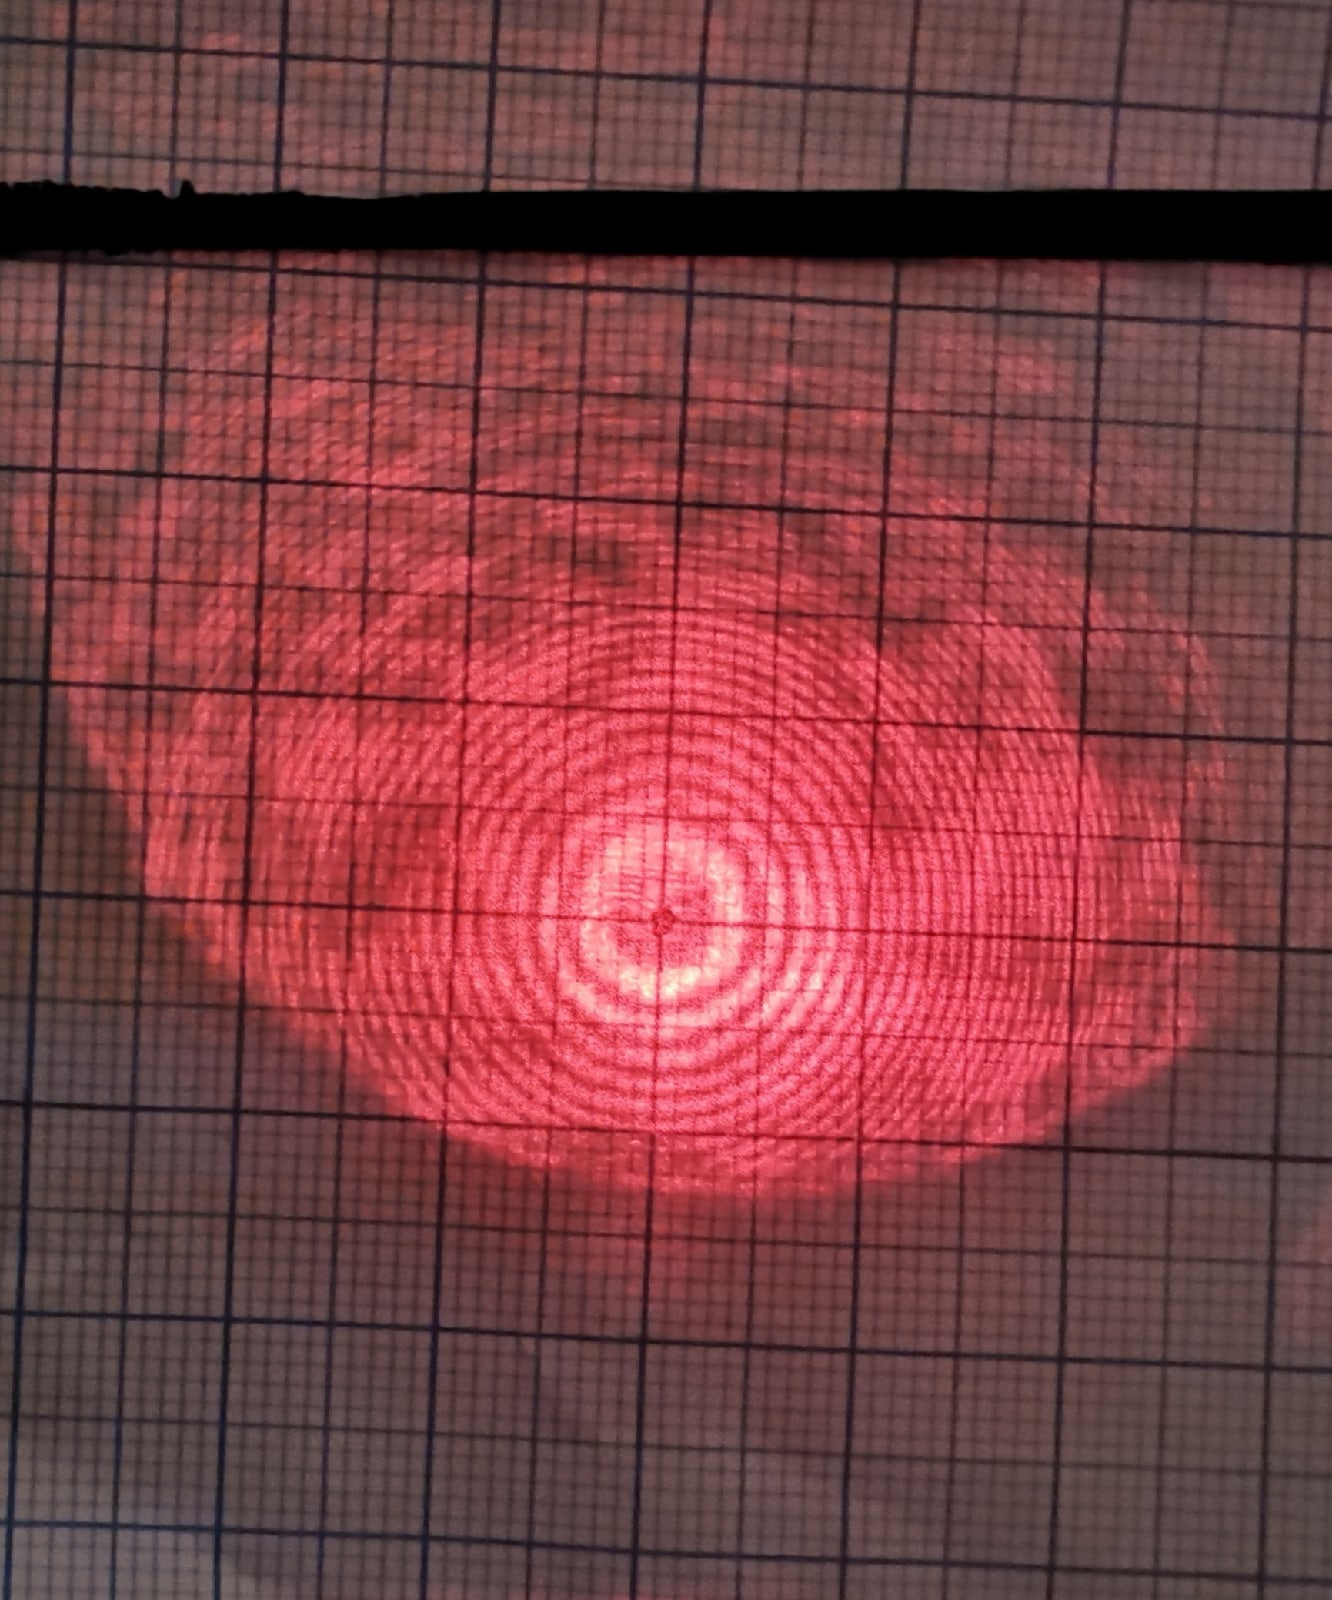
\includegraphics[width=\textwidth]{pics/rings.png}
        \caption{Наблюдение интерференционных колец}
    \end{minipage}
    \hfill
    \begin{minipage}[b]{0.4\textwidth}
  
        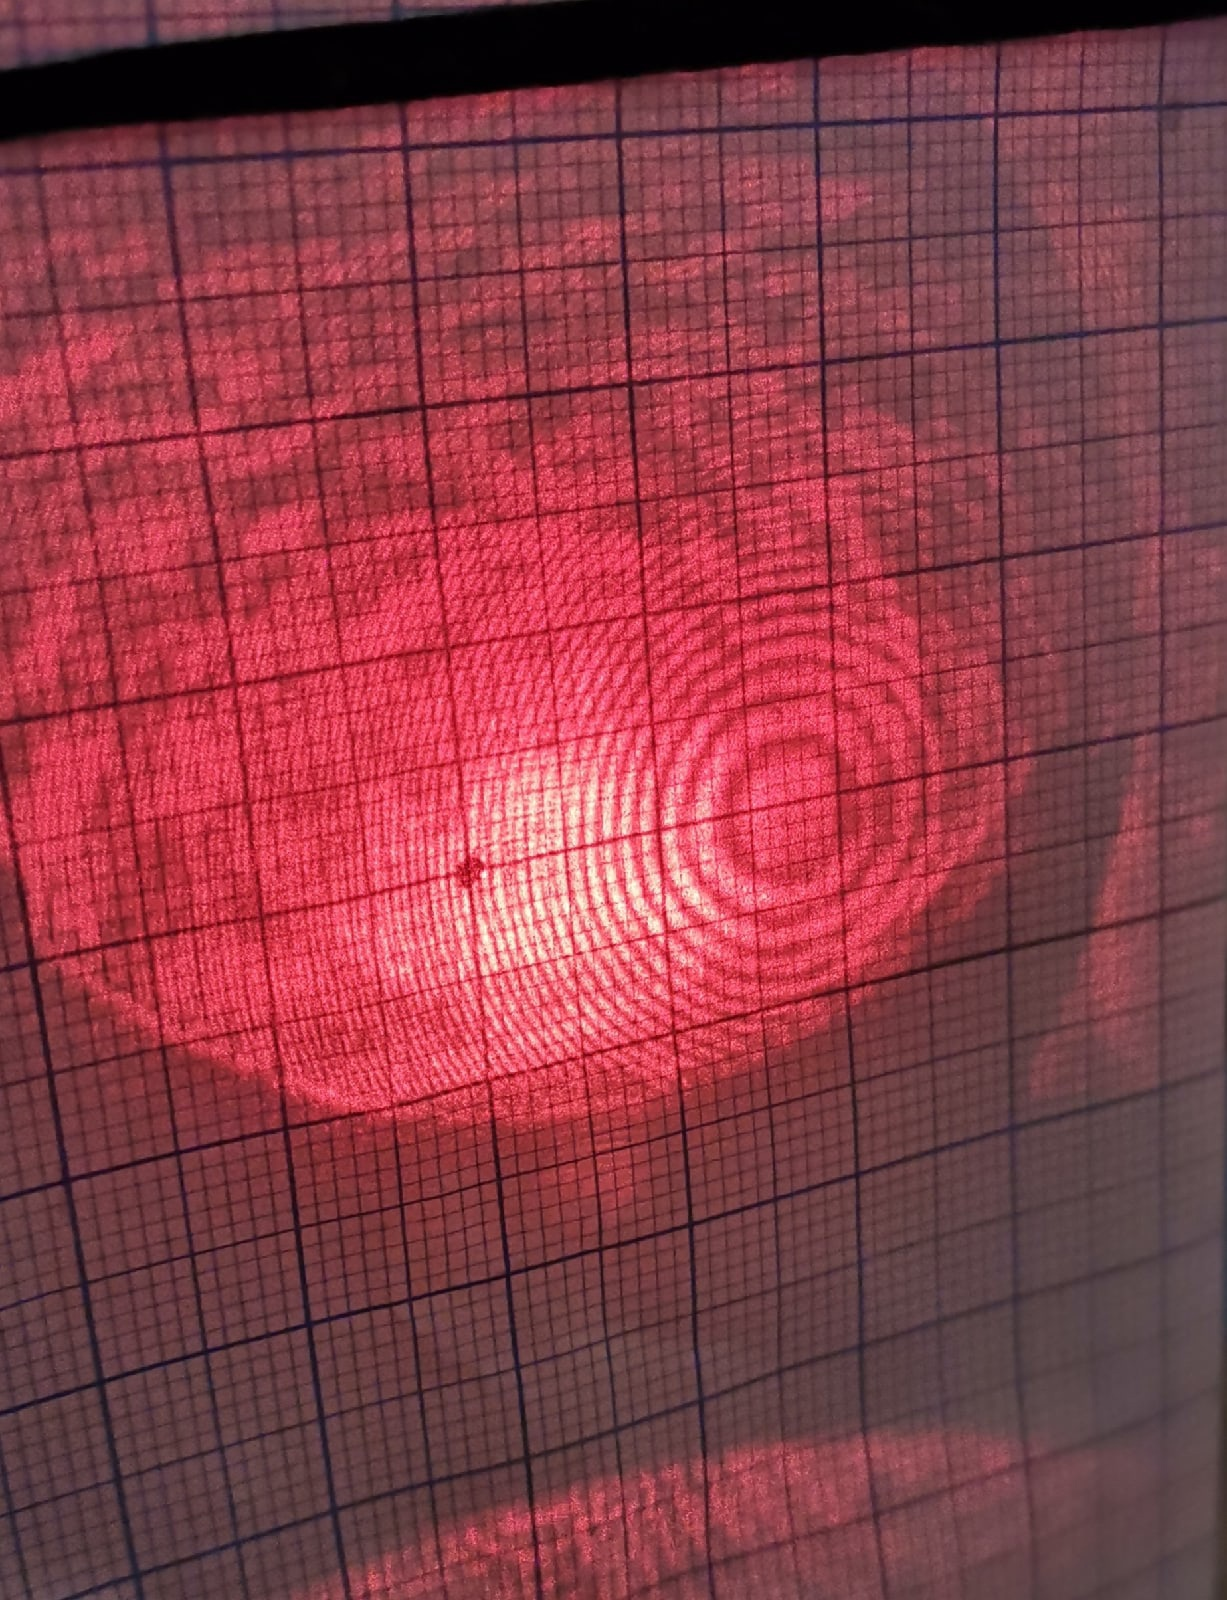
\includegraphics[width=\textwidth]{pics/stripes.png}
        \caption{Наблюдение интерференционной полосы}
      \end{minipage}    
    \end{figure}    
    
    
    \begin{table}[h!]
      \centering
      \begin{tabular}{| c | c | c | c | c | c | c |}
\hline
$n$ & $1$ & $2$ & $3$ & $4$ & $5$ & $6$\\
\hline
$r_n$ & $5$ & $7$ & $8$ & $9$ & $10$ & $11,5$\\
\hline
\end{tabular}

      \caption{}
      \label{nu1}
    \end{table}



\subsection{Измерение длины волны лазерного излучения}

Из таблицы получим среднее значение $N = 72101$ полос, за время 42.9 с (см. измерения в пункте 3). Тогда по формуле $v = \frac{\lambda N}{2T}$ , где $v = \frac{L}{T}$ легко получить длину волны лазера $\lambda = \frac{2L}{N} = 887.6$ нм

\begin{table}[h!]
	\centering
	\begin{tabular}{| c | c |}
\hline
$Iter., \: n$ & $Num \: of \: stripes, n$ \\
\hline 
$1$ & $63546$\\
\hline
$2$ & $61519$\\
\hline
$3$ & $71886$\\
\hline
$4$ & $67316$\\
\hline
$5$ & $79701$\\
\hline
$6$ & $82690$\\
\hline
$7$ & $65397$\\
\hline
$8$ & $85791$\\
\hline
$9$ & $85138$\\
\hline
$10$ & $58032$\\
\hline
\end{tabular}

	\caption{}
	\label{nu1}
\end{table}  


Из таблицы получим среднее значение $N = 72101$ полос, за время 42.9 с (см. измерения в пункте 3). Тогда по формуле $v = \frac{\lambda N}{2T}$ , где $v = \frac{L}{T}$ легко получить длину волны лазера $\lambda = \frac{2L}{N} = 887.6$ нм


\subsection{Исследование эффекта Доплера}

Для измерения длины лазерного излучения совместим центр интерференционной картины с отверстием в экране, и будем смотреть на показания частотомера в режиме счета импульсов.
Скорость двигателя установим на 1 (максимальную).
Как видно из полученной таблицы, количество прошедших через ФЭУ импульсов сильно отличается ввиду внешних колебаний системы.

Для измерения эффекта Доплера, сначала измерим время движения зеркала по измеряемому участку (L = 32 мм), откуда получим скорость движения зеркала, а затем проведем несколько (в нашем случае 6) измерений частоты колебания интенсивности света на ФЭУ при движении зеркала в каждую сторону.
Повторим измерения для трех разных скоростей двигателя.

Построим график разности частот при движении в разные стороны от квадрата скорости, откуда получаем угол наклона $\frac{\Delta \nu}{v^2} = 289 \cdot 10^{6}$ $\text{м}^{-2} $ с

При малых скоростях формула (1) позволяет нам выразить длину волны лазера
\begin{equation}
    N \pm \Delta N = 2\frac{vt}{\lambda}\frac{1}{1 \pm \frac{v}{c}}
\end{equation}

\begin{equation}
    \pm \Delta N = 2\frac{vt}{\lambda}(\mp \frac{v}{c})
\end{equation}


\begin{equation}
    \lambda = 4\frac{v^2}{\Delta \nu c}
\end{equation}

Таким образом получаем $\lambda = 2.3 \cdot 10^{-8}$ нм.

Результат, естественно, не совпадает длиной лазера ни в каком приближении. Такая большая ошибка происходит ввиду того, что эффект Доплера вносит поправку порядка отношения скорости к скорости света, которая в данном случае настолько мала, что на много порядков перекрывается погрешностями - т.е. мы наблюдаем разность частот обусловленную вибрацией установки, а следовательно не можем применять формулу, использованную нами для получения длины волны.

\begin{table}[h!]
	\centering
	\begin{tabular}{| c | c | c | c | c | c | c | c |}
    \hline
    
                     & $1$    & $2  $  &$ 3 $   & $4 $   & $5 $   & $6 $   & $\overline{\nu} $\\
    
    \hline
    
    $\nu, \rightarrow$ & 3000 & 2964 & 2877 & 2912 & 2888 & 2832 & 2912.2 \\
    
    \hline
    
    $\nu, \leftarrow$  & 2622 & 2562 & 2536 & 2564 & 2563 & 2592 & 2573.2\\
    
    \hline
    
    \multicolumn{8}{| c |}{Время движения зеркала: 42.9 с} \\
    
    \hline
    \end{tabular}
    
	\caption{Измерение номера дифракционной картины от координаты линзы}
	\label{nu1}
\end{table}

\begin{table}[h!]
	\centering
	\begin{tabular}{| c | c | c | c | c | c | c | c |}
    \hline
    
                     & $1  $  & $2 $   & $3 $   & $4 $   & $5 $   & $6 $   & $\overline{\nu} $\\
    
    \hline
    
    $\nu, \rightarrow $& 1233 & 1213 & 1246 & 1192 & 1222 & 1211 & 1219.5\\
    
    \hline
    
    $ \nu, \leftarrow $ & 1269 & 1254 & 1226 & 1249 & 1232 & 1230 & 1243.3\\
    
    \hline
    
    \multicolumn{8}{| c |}{Время движения зеркала: 82.6 с} \\
    
    \hline
    \end{tabular}
	\caption{Измерение номера дифракционной картины от координаты линзы}
	\label{nu1}
\end{table}

\begin{table}[h!]
	\centering
	\begin{tabular}{| c | c | c | c | c | c | c | c |}
    \hline
    
                     & $1 $   & $2 $   & $3 $   & $4 $   & $5 $   &$ 6 $   & $\overline{\nu}$ \\
    
    \hline
    
    $\nu, \rightarrow$ & 466 & 440 & 485 & 434 & 446 & 446 & 452.8 \\
    
    \hline
    
    $\nu, \leftarrow $ & 447 & 423 & 435 & 430 & 430 & 455 & 436,7 \\
    
    \hline
    
    \multicolumn{8}{| c |}{Время движения зеркала: 229.1 с} \\
    
    \hline
    \end{tabular}
	\caption{Измерение номера дифракционной картины от координаты линзы}
	\label{nu1}
\end{table}


\begin{figure}[h!]
  \centering
  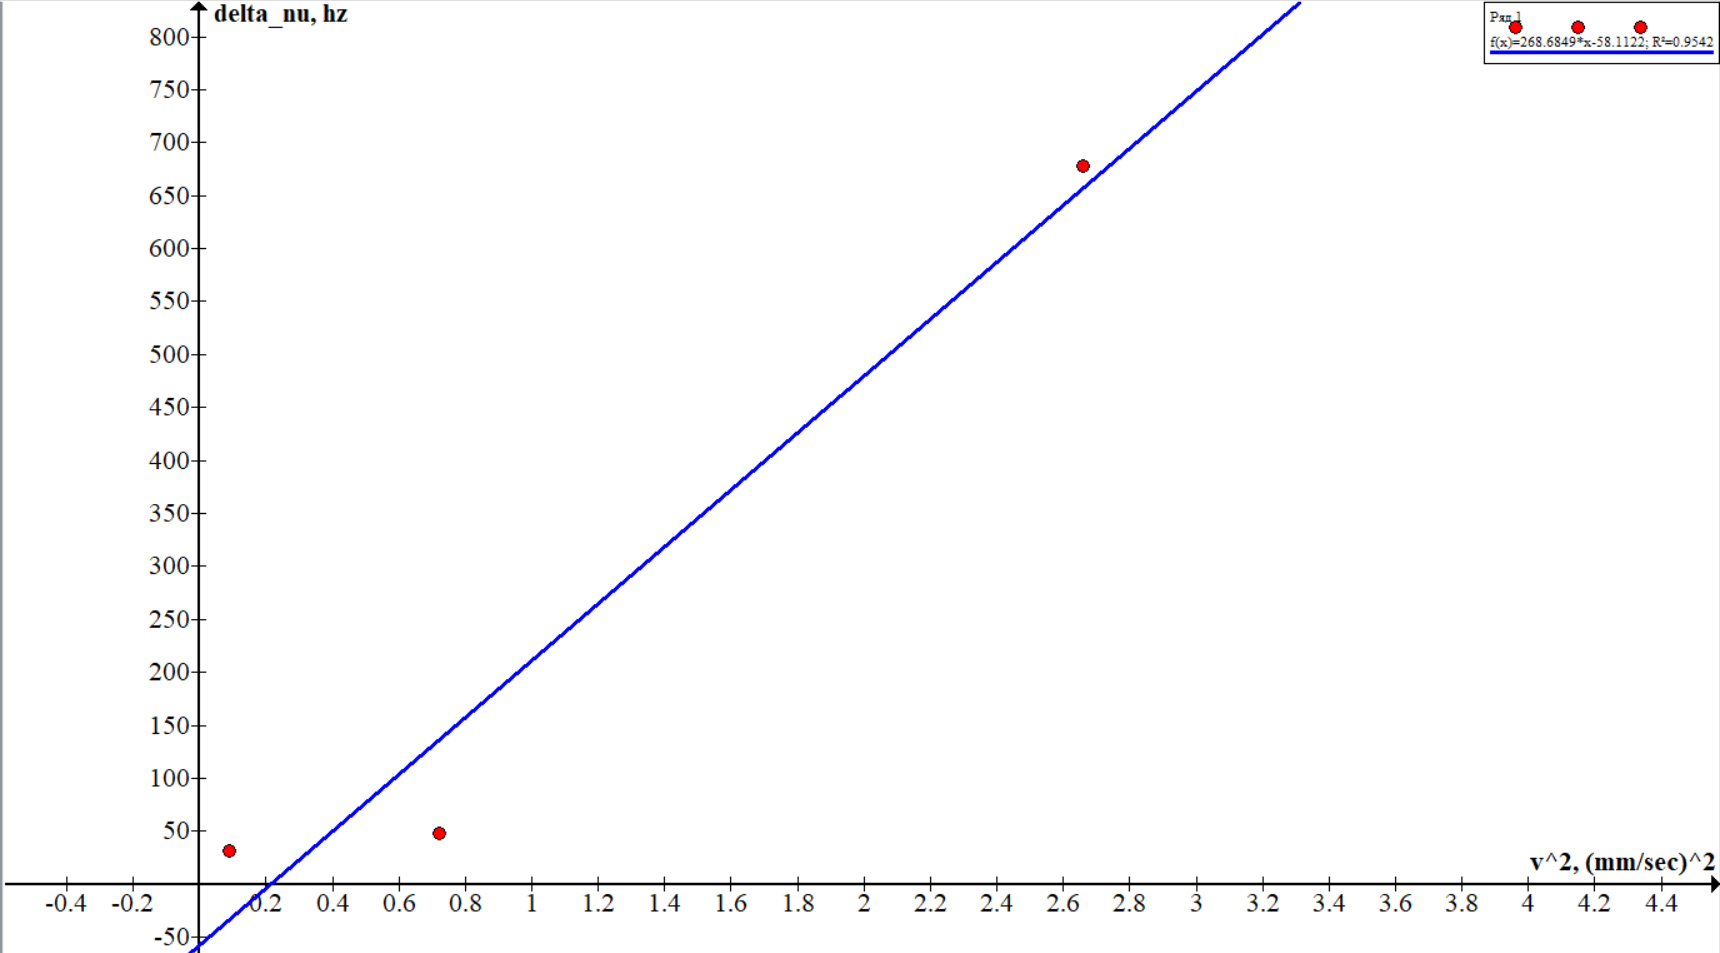
\includegraphics[width=1\linewidth]{pics/lab_4_2_4_2.png}
  \caption{Зависимость для анализа эффекта Доплера.}
  \label{}
\end{figure}

\subsection{Вывод}
Был изучен интерферометр Майкельсона, были проведены наблюдения интерференции на установке - как визуальные, так и с помощью ФЭУ. В данной работе основную часть погрешности вносит факт вибраций установки, который не мог быть устранен в рамках работы. Остальные погрешности либо пренебрежимо малы (как приборные погрешности), либо вносят несущественный вклад по сравнению c неидеальностью установки.

\end{document}